\clearpage
\begin{column}{ミニ研究}
\subsection*{ミニ研究：高尾駅周辺における自動運転オンデマンド交通の拠点配置分析}
{\small 名嘉山結月}

近年、自動運転オンデマンド交通は、鉄道や幹線バスを補完する端末交通として期待されている。
しかし、導入にあたっては、どの範囲を対象とするか、どこに拠点を置くか、どの程度の車両台数で需要をカバーできるかを検討する必要がある。
本ミニ研究では、高尾駅周辺3km圏を対象に、複数拠点配置と需要ゾーン割当を組み合わせた最適化モデルを構築し、サービス設計上の示唆を得ることを目的とした。

\paragraph{データと前提条件}
使用したのは2019年東京都市圏パーソントリップ調査データであり、高尾駅から半径3km圏に関係するトリップを抽出した。
対象需要は500mメッシュで集計し、各メッシュを需要ゾーンとして扱う。図\ref{fig:takao_mesh}に対象地域と500mメッシュ需要分布を示す。
需要量 $d_i$ はゾーンごとに算出し、高齢者や免許非保有、自由に使える自動車の有無、外出困難、高齢者同行などをもとに公平性指標 $fairness\_ratio$ *を設定した。
潜在需要は需要量の20\%と仮定した。
高尾駅を主拠点とし、追加拠点候補は3km圏内を空間的に分散してカバーするように設定している。

% 図を入れる場合
 \begin{center}
   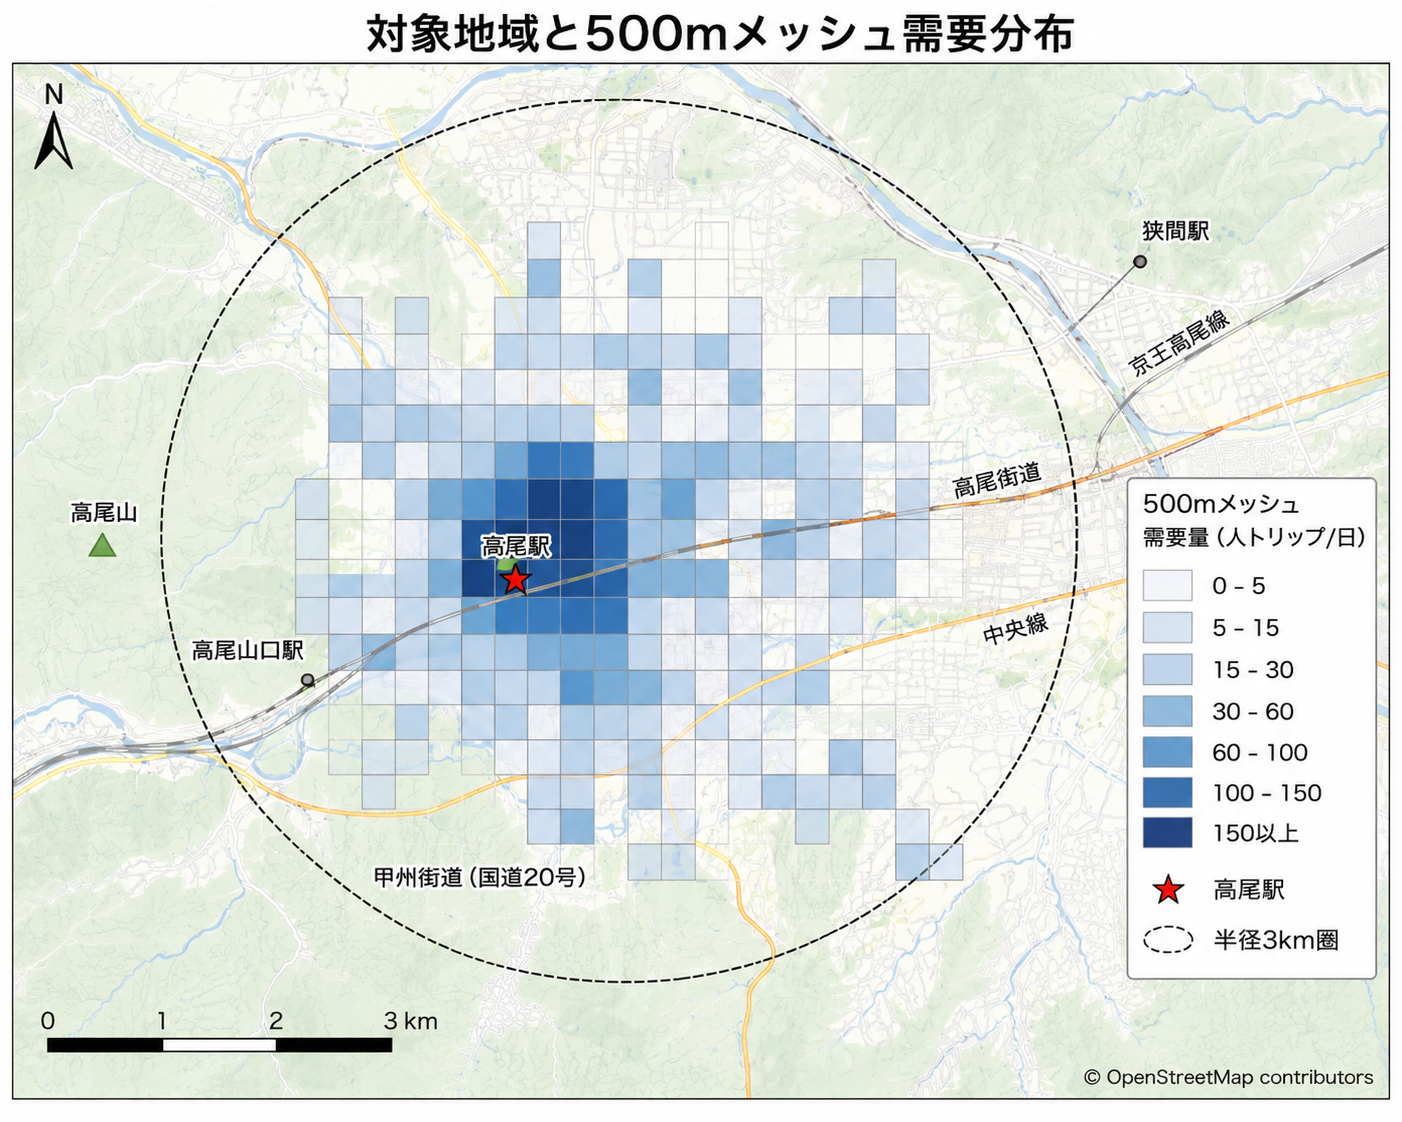
\includegraphics[width=\linewidth]{assets/optimization/optimization/column/fig_mesh_demand.png}
   \captionof{figure}{対象地域と500mメッシュ需要分布}
   \label{fig:takao_mesh}
 \end{center}

*公平性指標は、各個人の支援必要度をもとにゾーン単位で集計した。

\[
s_i = w_1 E_i + w_2 L_i + w_3 C_i + w_4 D_i + w_5 A_i
\]

\[
fairness\_ratio_z
=
\frac{1}{N_z}
\sum_{i \in z} s_i
\]

ここで、
$E_i$ は高齢者、
$L_i$ は免許非保有、
$C_i$ は自由に使える自動車なし、
$D_i$ は外出困難、
$A_i$ は高齢者同行
を表す0/1変数である。
なお、本分析における fairness\_ratio は厳密な福祉指標ではなく、移動制約のある需要を相対的に重視するための proxy として扱っている。
\paragraph{初期分析：3種類のサービス設計}
まず、設計思想の違いを比較するため、以下の3種類のモデルを比較した。

\begin{itemize}
  \item ① 半径型（radius）：高尾駅から一定距離圏内を一括してサービス対象とする。実装容易性を重視した単純な構造。
  \item ② 分散型（demand-based）：需要の大きいゾーンを個別に選択し、効率性を重視する構造。
  \item ③ カバー率型（coverage）：一定割合以上の需要を必ずカバーし、公平性・公共性を重視する構造。
\end{itemize}

比較の結果、カバー率を高めるほどサービス時間が増加し、効率性と公平性の間に明確なトレードオフが存在することが確認された。
また、需要の大きいゾーンを優先する分散型では効率性が高い一方、空間的な偏りが生じやすいことが示唆された。表\ref{tab:results_comparison}に3種類のサービス設計比較を示す。

% 表を入れる場合
 \begin{center}
   \begin{tabular}{lll}
     \toprule
     モデル & 特徴 & 主な示唆 \\
     \midrule
     半径型 & 実装容易性重視 & シンプルだが公平性が不明確 \\
     分散型 & 効率性重視 & 需要偏在で空間的偏りが生じやすい \\
     カバー率型 & 公共性重視 & coverage 増加で service time が増加 \\
     \bottomrule
   \end{tabular}
   \captionof{table}{最適化結果比較}
   \label{tab:results_comparison}
 \end{center}

\paragraph{モデル化}
今回は、本格的なVRPではなく、複数拠点配置＋需要ゾーン割当問題として定式化した。
各需要ゾーンは、選択された拠点のいずれかに割り当てられる。
高尾駅は必ず使用する拠点とし、追加拠点を候補集合から選択する。

サービス時間は、拠点からゾーンへの往復時間に加えて、乗降・待機バッファおよび高尾駅との接続コストを含む近似値として定義した。

\[
t_{ij}
=
2 \times \frac{l_{ij}}{v} \times 60
+
b
+
\gamma \times \frac{h_j}{v} \times 60
\]

ここで、
$l_{ij}$ は拠点 $j$ からゾーン $i$ までの距離[km]、
$v$ は平均速度[km/h]、
$b$ は乗降・待機バッファ[min]、
$h_j$ は拠点 $j$ と高尾駅との距離[km]、
$\gamma$ は駅接続コストの重みである。

この式は、端末交通として各拠点が高尾駅と接続される必要性を近似的に表現したものである。

解法には0-1整数計画（MILP）を用い、目的関数は総サービス時間の最小化とした。

決定変数は以下のとおりである。

\[
x_j = 
\begin{cases}
1 & \text{拠点 } j \text{ を使用する場合} \\
0 & \text{それ以外}
\end{cases}, \qquad
y_{ij} =
\begin{cases}
1 & \text{ゾーン } i \text{ を拠点 } j \text{ に割り当てる場合} \\
0 & \text{それ以外}
\end{cases}
\]

ここで、
$d_i$ はゾーン $i$ の有効需要（effective demand）、
$t_{ij}$ は拠点 $j$ がゾーン $i$ を担当する場合のサービス時間[min]、
$y_{ij}$ はゾーン $i$ を拠点 $j$ に割り当てるかを表す0/1変数である。
なお、繰り返しになるが、有効需要は各ゾーン需要の20\%と仮定した。
また、
$f_i$ はゾーン $i$ の公平性指標、
$C_j$ は拠点 $j$ の処理可能容量を表す。

目的関数は次の形を想定した。

\[
\min \sum_i \sum_j d_i t_{ij} y_{ij}
\]


制約としては、以下の通り、coverage 制約、fairness 制約、拠点数制約、容量制約、割当制約を設定した。

\begin{align*}
&\sum_i d_i z_i \ge \alpha \sum_i d_i
&& \text{(coverage 制約)} \\
&\sum_i d_i f_i z_i \ge \beta \sum_i d_i f_i
&& \text{(fairness 制約)} \\
&\sum_j x_j = P
&& \text{(拠点数制約)} \\
&\sum_j y_{ij} \le 1
&& \forall i \quad \text{(割当制約)} \\
&y_{ij} \le x_j
&& \forall i,j \\
&\sum_i d_i t_{ij} y_{ij}
\le
C_j x_j
&& \forall j \quad \text{(容量制約)}
\end{align*}

\paragraph{計算条件}
高尾駅は必須拠点とし、追加拠点数 $P$ を変化させる。
coverage threshold は 0.4、0.5、0.6 を比較し、総車両台数 fleet を変更した。
さらに、nearest-$k$ 制約を導入し、$k=1$ に近づくほど各拠点の担当圏域が独立する条件を検討した。

% 表を入れる場合
 \begin{center}
   \begin{tabular}{ll}
     \toprule
     項目 & 内容 \\
     \midrule
     対象地域 & 高尾駅周辺3km圏 \\
     需要単位 & 500mメッシュ \\
     effective demand & demand の20\% \\
　　　fleet & 18 / 24 \\ 
     必拠点 & 高尾駅 \\
     追加拠点数 $P$ & 1-4 \\
     coverage threshold & 0.4, 0.5, 0.6 \\
     fairness\_threshold & 0.3 \\ 
     nearest-$k$ 制約 & $k=1$ に近い条件 \\
     \bottomrule
   \end{tabular}
   \captionof{table}{主要パラメータ一覧}
   \label{tab:parameters}
 \end{center}


\paragraph{計算結果}
最適解の一例として、$P=3$ の場合には「高尾駅 + candidate\_6 + candidate\_8」が選択された。図\ref{fig:optimal_locations}に最適拠点配置結果を示す。
このとき、coverage は約0.5、capacity utilization は約1.0 となり、車両容量制約が強く効いていることが確認された。
図\ref{fig:tradeoff}に示すように，coverage を高めると総サービス時間が大きく増加し、効率性と公共性のトレードオフが確認された。
また、fleet 数を減少させた場合には、coverage 制約を満たす解が存在しない infeasible ケースが確認された。
これは、自動運転オンデマンド交通の成立性が、需要量だけでなく投入可能な車両規模にも強く依存することを示している。
一方で、fleet 数を増加させても、拠点配置や coverage 条件が同一である場合には、総サービス時間の改善は限定的であった。
したがって、fleet 数は「効率性」よりも「サービス成立性」を左右する要因として機能したと考えられる。

% 図を入れる場合
 \begin{center}
   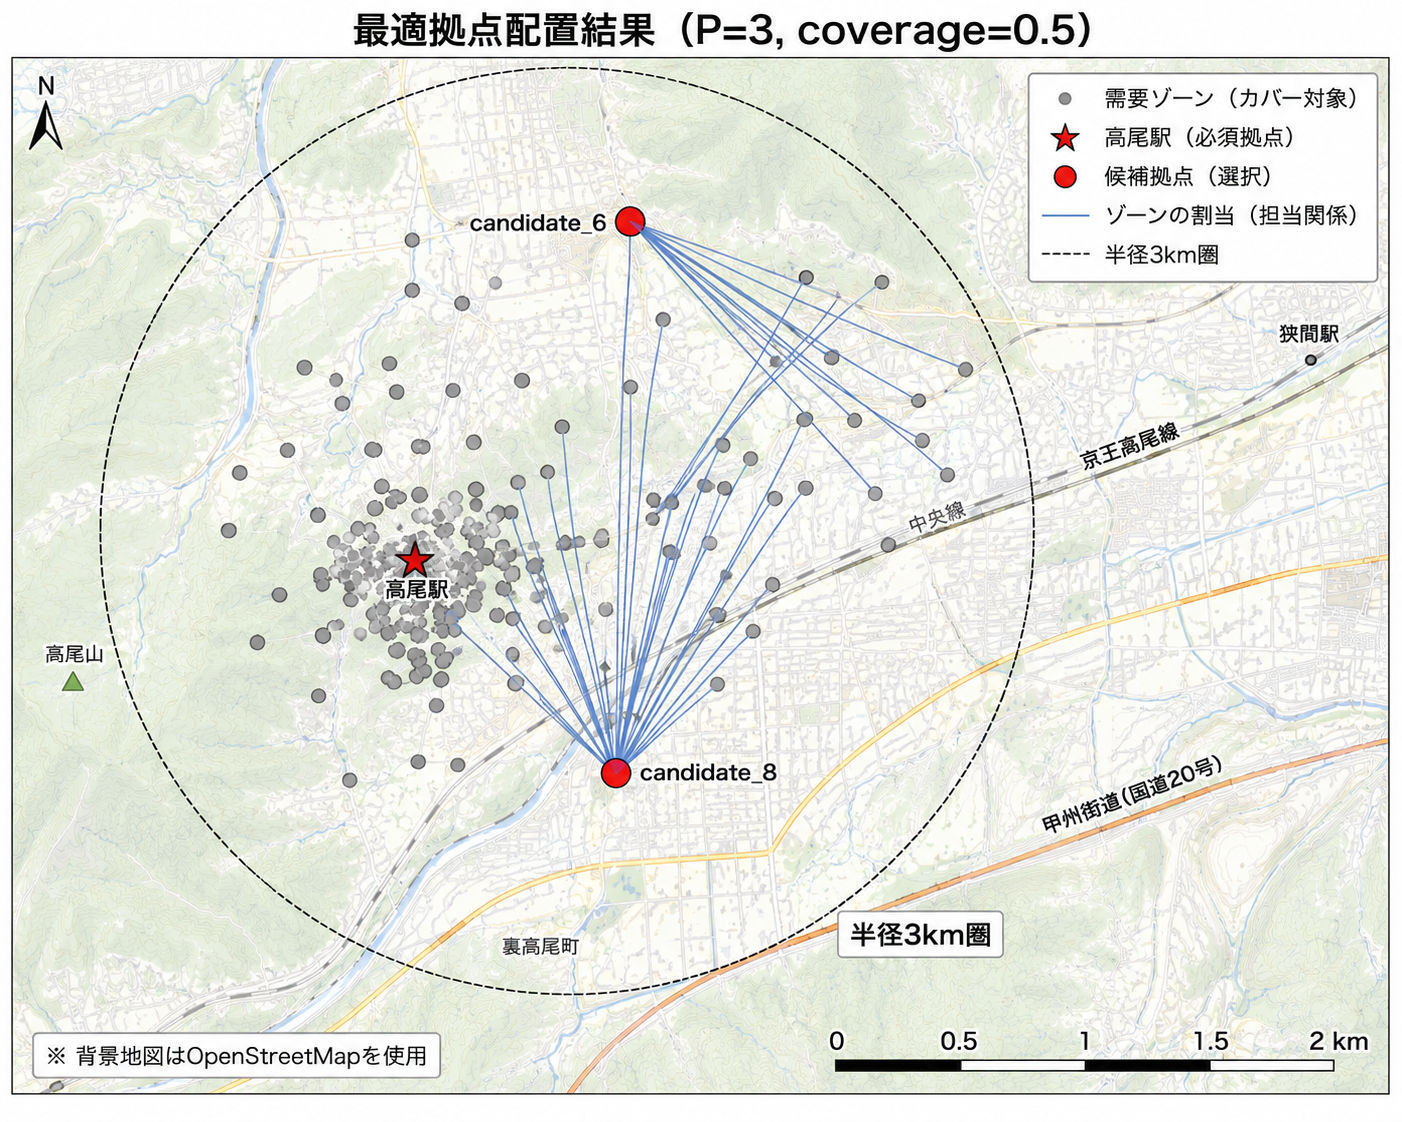
\includegraphics[width=\linewidth]{assets/optimization/optimization/column/fig_optimal_hubs.png}
   \captionof{figure}{最適拠点配置結果}
   \label{fig:optimal_locations}
 \end{center}

% 図を入れる場合
 \begin{center}
   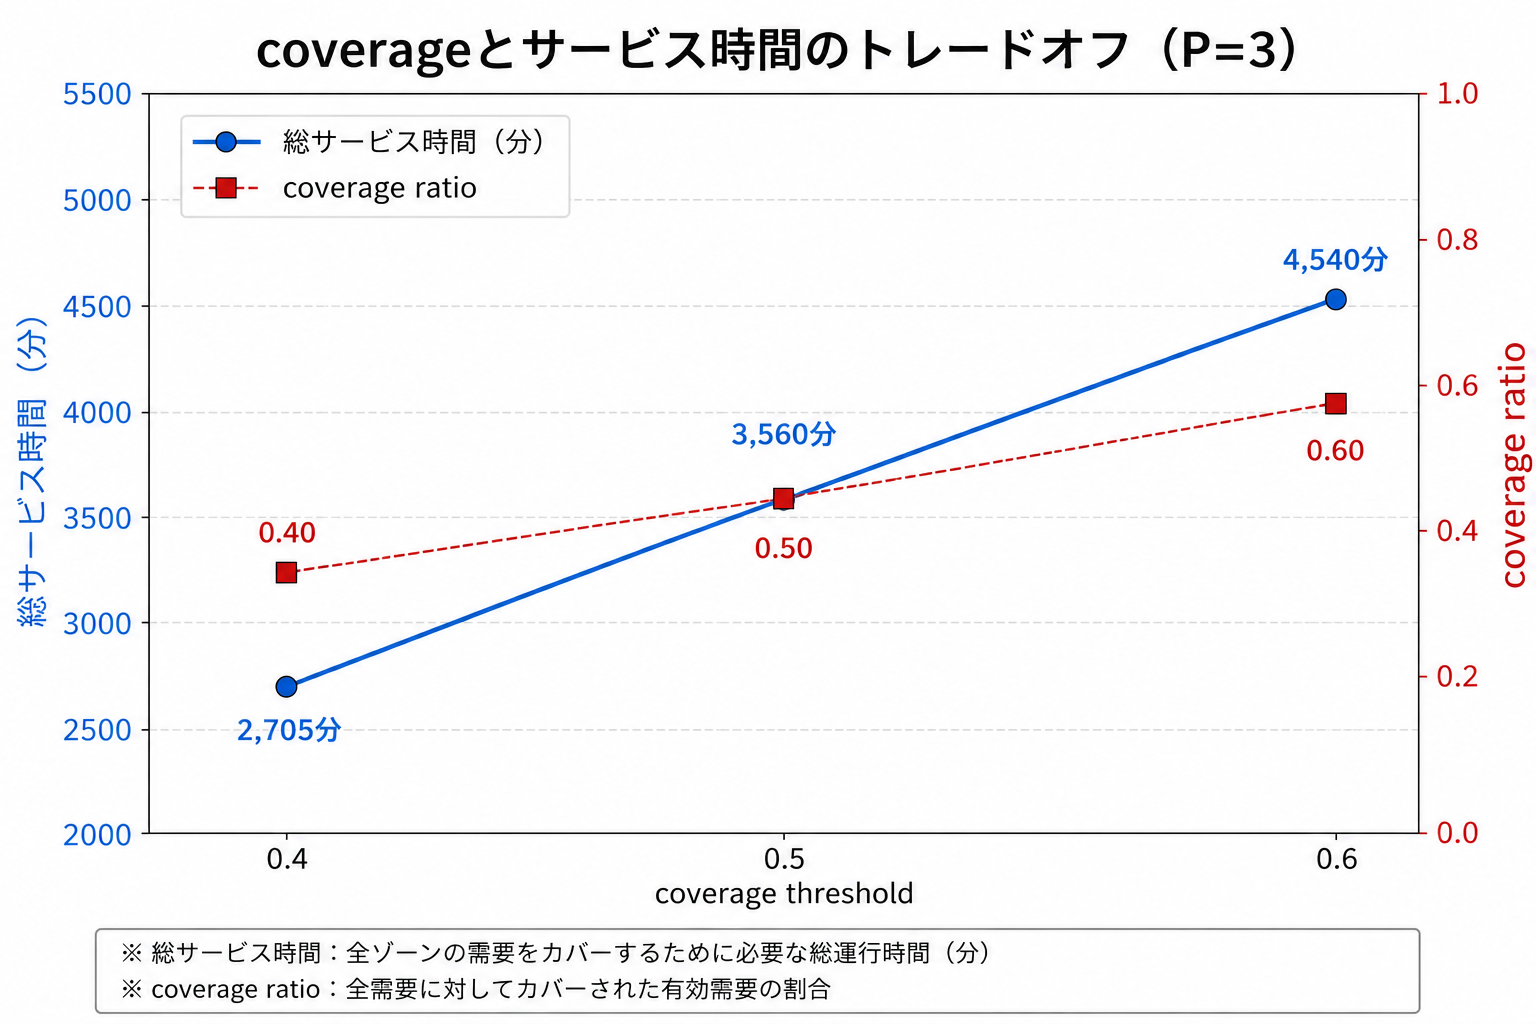
\includegraphics[width=\linewidth]{assets/optimization/optimization/column/fig_tradeoff.png}
   \captionof{figure}{coverage と service time のトレードオフ}
   \label{fig:tradeoff}
 \end{center}

\begin{center}
\begin{tabular}{lrrrrr}
\toprule
ケース & 選択拠点数 & coverage\_ratio & fairness\_coverage\_ratio & total\_service\_time\_min & capacity\_utilization\_mean \\ 
\midrule
P1\_k8 & 1 & 0.5 & 0.526 & 3006.6 & 0.651 \\ 
P2\_k8 & 2 & 0.5 & 0.517 & 3167.1 & 0.651 \\ 
P3\_k8 & 3 & 0.5 & 0.515 & 3633.2 & 0.651 \\ 
P4\_k8 & 4 & 0.5 & 0.511 & 3884.2 & 0.732 \\ 
cov40\_k8 & 3 & 0.4 & 0.4 & 2805.2 & 0.52 \\ 
cov50\_k8 & 3 & 0.5 & 0.515 & 3633.2 & 0.651 \\ 
cov60\_k8 & 3 & 0.6 & 0.618 & 4407.1 & 0.781 \\ 
beta00\_k8 & 3 & 0.5 & 0.515 & 3633.2 & 0.651 \\ 
beta05\_k8 & 3 & 0.5 & 0.515 & 3633.2 & 0.651 \\ 
beta10\_k8 & 3 & 0.5 & 0.515 & 3633.2 & 0.651 \\ 
\bottomrule
\end{tabular}
\captionof{table}{最適化結果比較}
\label{tab:results}
\end{center}

\paragraph{分析と考察}
本分析では、表\ref{tab:results}に示す通り、拠点数 $P$ を増加させても効率性が大きく改善するとは限らず、むしろ coverage の設定や車両容量制約が支配的であることが示された。
一般には拠点数を増やすことで各ゾーンまでの距離が短縮される可能性があるが、本分析では、追加拠点と高尾駅との接続コストや coverage 制約の影響により、総サービス時間が必ずしも減少しなかった。
したがって、単に拠点数を増加させるのではなく、拠点配置と担当圏域を一体的に設計する必要があると考えられる。

都市部では需要密度が高いため、「どこをカバーするか」よりも「限られた車両容量でどれだけ効率的に運用できるか」が主要な制約となる可能性がある。
一方、地方部では需要分布がより分散するため、拠点配置そのものが支配的な問題となることが考えられる。

\paragraph{今後の展望}
本分析を発展させるためには、道路ネットワークを用いた厳密なルーティングや公共施設を考慮した拠点配置、nearest-$k$ 制約の厳密化が求められる。
さらに、地方部への展開や避難・物流との統合的分析も今後の課題である。
\end{column}
\clearpage
